\scanpage{138}
\begin{center}\reflectbox{\begin{minipage}{.95\linewidth}\ttfamily\scriptsize\color{gray}
\unsure{PAGE 1\quad ON=CELMPQRSTV\quad08/19/82-15:20:31\quad CFT 1.09(06/28/82)\quad PAGE 1}\par
\unsure{1\quad1.\quad PROGRAM CRAY7}\par
\unsure{2\quad2.\quad WRITE(6,1)}\par
\unsure{3\quad3.\quad1 FORMAT(' BONJOUR')}\par
\unsure{4\quad4.\quad STOP}\par
\unsure{5\quad5.\quad END}
\end{minipage}}\end{center}
\figure{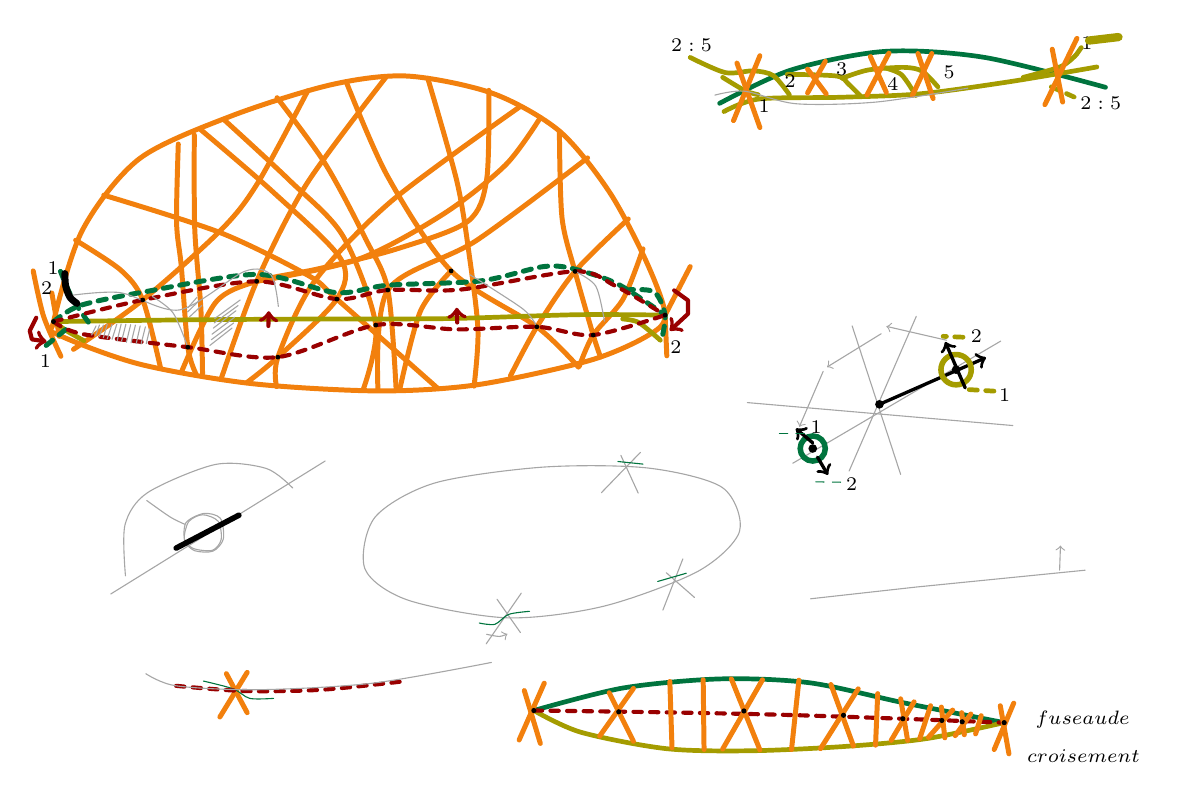
\begin{tikzpicture}[x=.55cm,y=-.55cm,line cap=round,line join=round,g/.style={olive!80!yellow,line width=1.7pt},r/.style={orange!80!brown,line width=1.8pt},w/.style={red!60!black,line width=1.5pt},b/.style={blue!60!black,line width=1.4pt},p/.style={gray!70,thin},k/.style={black,line width=1.2pt},every node/.style={font=\scriptsize}]
% Small upper-right strip and numbered sectors.
\draw[blue!35!green!70!black,line width=1.7pt] plot[smooth] coordinates {(17.87,2.74) (19.52,1.97) (21.69,1.54) (23.99,1.68) (26.78,2.37)};
\draw[g] plot[smooth] coordinates {(17.97,2.93) (18.78,2.64) (20.66,2.6) (22.5,2.52) (24.57,2.24) (26.58,1.9)};
\draw[g] plot[smooth] coordinates {(17.19,1.68) (18.0,2.03) (18.65,1.99) (19.11,2.1) (19.48,2.54)};
\draw[g] plot[smooth] coordinates {(17.94,2.14) (18.46,2.45) (18.76,2.54)};
\draw[g] plot[smooth] coordinates {(19.43,2.07) (20.57,2.11) (20.84,2.29) (21.13,2.58)};
\draw[g] plot[smooth] coordinates {(20.7,2.16) (21.3,1.97) (22.13,1.91) (22.55,2.0) (22.91,2.36)};
\draw[g] plot[smooth] coordinates {(21.68,1.92) (22.07,2.08) (22.4,2.56)};
\draw[g] plot[smooth] coordinates {(24.88,2.14) (25.75,1.89) (26.1,1.62)};
\draw[g,dashed] plot[smooth] coordinates {(25.53,2.36) (26.18,2.65)};
\draw[g,dashed] plot[smooth] coordinates {(26.11,1.61) (26.32,1.31)};
\draw[r] plot[smooth] coordinates {(18.27,1.81) (18.8,3.3)};
\draw[r] plot[smooth] coordinates {(18.8,1.64) (18.19,3.14)};
\draw[r] plot[smooth] coordinates {(19.9,1.95) (20.33,2.52)};
\draw[r] plot[smooth] coordinates {(20.31,1.77) (19.9,2.5)};
\draw[r] plot[smooth] coordinates {(21.35,1.66) (21.72,2.49)};
\draw[r] plot[smooth] coordinates {(21.78,1.58) (21.27,2.55)};
\draw[r] plot[smooth] coordinates {(22.45,1.59) (22.8,2.63)};
\draw[r] plot[smooth] coordinates {(22.77,1.59) (22.32,2.56)};
\draw[r] plot[smooth] coordinates {(25.55,1.49) (25.79,2.71)};
\draw[r] plot[smooth] coordinates {(26.12,1.24) (25.38,2.77)};
\draw[p] plot[smooth] coordinates {(17.76,2.55) (18.45,2.46) (19.64,2.75) (21.49,2.71) (23.6,2.39)};
\node at (17.22,1.39) {$2:5$};
\node at (18.9,2.8) {$1$};
\node at (19.5,2.24) {$2$};
\node at (20.69,1.95) {$3$};
\node at (21.87,2.29) {$4$};
\node at (23.17,2.02) {$5$};
\node at (26.35,1.35) {$1$};
\node at (26.67,2.73) {$2:5$};
\draw[g,line width=3pt] (26.4,1.29)--(27.08,1.21);
% Large orange bounded arrangement: all crossing curves and marked intersections.
\draw[r] plot[smooth cycle] coordinates {(2.49,7.78) (3.16,5.66) (4.47,4.02) (6.6,3.03) (8.9,2.31) (10.66,2.11) (12.63,2.51) (14.17,3.38) (15.32,4.78) (16.18,6.4) (16.61,7.63) (16.2,8.11) (14.86,8.68) (12.26,9.24) (9.97,9.38) (7.05,9.21) (4.47,8.76) (2.59,8.08)};
\draw[r] plot[smooth] coordinates {(3.0,5.9) (4.04,6.59) (4.55,7.28) (4.96,8.85)};
\draw[r] plot[smooth] coordinates {(3.65,4.86) (6.35,5.73) (8.38,6.72) (9.03,7.26) (11.36,9.32)};
\draw[r] plot[smooth] coordinates {(5.37,3.68) (5.33,5.49) (5.44,6.51) (5.59,8.37) (5.78,8.99)};
\draw[r] plot[smooth] coordinates {(5.74,3.47) (5.75,5.64) (5.89,7.46) (5.93,8.99)};
\draw[r] plot[smooth] coordinates {(5.89,3.35) (7.55,4.78) (9.12,6.33) (9.03,7.26) (7.67,8.6) (6.95,9.19)};
\draw[r] plot[smooth] coordinates {(6.44,3.13) (7.94,4.52) (9.17,5.8) (9.93,7.86) (9.64,9.35)};
\draw[r] plot[smooth] coordinates {(7.65,2.61) (8.76,4.13) (9.69,5.86) (10.21,7.05) (10.4,9.35)};
\draw[r] plot[smooth] coordinates {(8.36,2.45) (7.21,4.57) (6.37,5.65) (4.55,7.28) (2.95,8.42)};
\draw[r] plot[smooth] coordinates {(9.25,2.25) (10.2,4.42) (11.67,6.61) (13.65,7.9) (14.61,8.83)};
\draw[r] plot[smooth] coordinates {(10.17,2.13) (8.34,4.59) (7.18,6.85) (6.36,9.1)};
\draw[r] plot[smooth] coordinates {(11.13,2.16) (11.81,4.57) (12.1,6.33) (12.29,7.99) (12.2,9.27)};
\draw[r] plot[smooth] coordinates {(12.54,2.44) (12.49,4.5) (12.05,5.47) (10.42,6.1) (8.61,6.56) (7.18,6.85) (6.23,7.34) (5.44,8.95)};
\draw[r] plot[smooth] coordinates {(13.27,2.81) (10.3,4.99) (8.5,6.87) (7.67,8.6) (7.64,9.28)};
\draw[r] plot[smooth] coordinates {(13.73,3.07) (12.93,4.16) (11.5,5.29) (9.53,6.34) (7.18,6.85)};
\draw[r] plot[smooth] coordinates {(14.17,3.38) (14.23,5.38) (14.53,6.62) (14.95,8.09) (15.12,8.6)};
\draw[r] plot[smooth] coordinates {(14.82,4.0) (12.25,5.91) (10.21,7.05) (9.98,9.35)};
\draw[r] plot[smooth] coordinates {(15.76,5.41) (14.53,6.62) (13.65,7.9) (13.04,9.03)};
\draw[r] plot[smooth] coordinates {(16.1,6.1) (15.64,7.26) (14.95,8.09) (14.63,8.81)};
\draw[r] plot[smooth] coordinates {(11.67,6.61) (10.96,7.54) (10.48,9.36)};
\draw[r] plot[smooth] coordinates {(2.02,6.61) (2.26,7.66) (2.66,8.58)};
\draw[r] plot[smooth] coordinates {(2.45,7.12) (2.56,7.75) (2.62,8.12)};
\draw[r] plot[smooth] coordinates {(16.61,7.63) (17.19,6.51)};
\draw[r] plot[smooth] coordinates {(16.61,7.63) (16.65,8.57)};
\draw[g] plot[smooth] coordinates {(2.49,7.78) (5.53,7.74) (8.53,7.72) (11.6,7.71) (14.6,7.62) (16.61,7.63)};
\draw[g] plot[smooth] coordinates {(2.49,7.78) (2.82,8.01) (3.19,8.22)};
\draw[g] plot[smooth] coordinates {(15.63,7.72) (16.0,7.8) (16.5,8.21)};
\draw[blue!35!green!70!black,line width=1.8pt,dashed] plot[smooth] coordinates {(2.49,7.78) (3.1,7.41) (4.55,7.1) (7.18,6.69) (9.01,7.11) (10.21,6.94) (12.35,6.84) (13.8,6.51) (14.53,6.57) (15.53,6.92) (16.61,7.63)};
\draw[blue!35!green!70!black,line width=1.8pt,dashed] plot[smooth] coordinates {(2.65,6.62) (2.93,7.26) (3.35,7.87)};
\draw[blue!35!green!70!black,line width=1.8pt,dashed] plot[smooth] coordinates {(2.32,8.33) (2.87,7.88)};
\draw[blue!35!green!70!black,line width=1.8pt,dashed] plot[smooth] coordinates {(15.69,7.05) (16.35,7.09) (16.61,7.63) (16.52,8.24)};
\draw[w,dashed] plot[smooth] coordinates {(2.49,7.78) (4.55,7.28) (7.18,6.85) (9.03,7.26) (10.21,7.05) (11.89,7.04) (14.53,6.62) (15.47,6.96) (16.61,7.63)};
\draw[w,dashed] plot[smooth] coordinates {(2.49,7.78) (3.17,8.07) (5.59,8.37) (7.67,8.6) (9.93,7.86) (11.79,7.96) (13.65,7.9) (14.95,8.09) (16.61,7.63)};
\draw[p] plot[smooth] coordinates {(2.85,7.18) (4.02,7.11) (5.4,7.51) (6.9,6.62) (7.51,6.7) (7.68,7.43)};
\draw[p] plot[smooth] coordinates {(4.77,7.2) (5.25,7.58) (5.59,8.37)};
\draw[p] plot[smooth] coordinates {(12.11,6.7) (13.33,7.49) (13.65,7.9)};
\draw[p] plot[smooth] coordinates {(14.53,6.62) (15.01,6.96) (15.21,7.77)};
\draw[p] (3.47,7.88)--(3.37,8.09);
\draw[p] (3.55,7.86)--(3.46,8.1);
\draw[p] (3.64,7.86)--(3.55,8.12);
\draw[p] (3.73,7.84)--(3.64,8.15);
\draw[p] (3.84,7.84)--(3.73,8.18);
\draw[p] (3.95,7.84)--(3.84,8.19);
\draw[p] (4.05,7.84)--(3.96,8.22);
\draw[p] (4.16,7.84)--(4.06,8.23);
\draw[p] (4.27,7.85)--(4.17,8.26);
\draw[p] (4.38,7.86)--(4.28,8.27);
\draw[p] (4.49,7.88)--(4.4,8.28);
\draw[p] (4.61,7.9)--(4.51,8.3);
\draw[p] (4.71,7.95)--(4.63,8.29);
\draw[p] (5.59,7.46)--(5.8,7.22);
\draw[p] (5.58,7.56)--(5.86,7.29);
\draw[p] (5.63,7.67)--(5.91,7.41);
\draw[p] (6.21,7.71)--(6.8,7.28);
\draw[p] (6.2,7.81)--(6.75,7.41);
\draw[p] (6.18,7.93)--(6.7,7.53);
\draw[p] (6.15,8.07)--(6.67,7.68);
\draw[p] (6.13,8.2)--(6.65,7.81);
\draw[p] (6.1,8.33)--(6.61,7.93);
\draw[k,line width=2.5pt] plot[smooth] coordinates {(2.75,6.67) (2.77,6.96) (2.87,7.22) (3.03,7.36)};
\draw[w,->] (2.09,7.69)--(1.94,7.99)--(1.99,8.19)--(2.33,8.24);
\draw[w,->] (16.82,7.06)--(17.14,7.29)--(17.14,7.6)--(16.72,7.99);
\draw[w,->] (7.45,7.88)--(7.46,7.54);
\draw[w,->] (11.81,7.8)--(11.8,7.46);
\fill[black] (2.49,7.78) circle (.055);
\fill[black] (4.55,7.28) circle (.055);
\fill[black] (5.59,8.37) circle (.055);
\fill[black] (7.18,6.85) circle (.055);
\fill[black] (7.67,8.6) circle (.055);
\fill[black] (9.03,7.26) circle (.055);
\fill[black] (9.93,7.86) circle (.055);
\fill[black] (10.21,7.05) circle (.055);
\fill[black] (11.67,6.61) circle (.055);
\fill[black] (13.65,7.9) circle (.055);
\fill[black] (14.53,6.62) circle (.055);
\fill[black] (14.95,8.09) circle (.055);
\fill[black] (16.61,7.63) circle (.055);
\node at (2.3,8.69) {$1$};
\node at (2.33,7.01) {$2$};
\node at (2.48,6.54) {$1$};
\node at (16.86,8.38) {$2$};
% Middle-right oriented radial drawing with two coloured circled points.
\draw[p] (20.93,7.88)--(22.05,11.31);
\draw[p] (22.41,7.66)--(20.86,11.23);
\draw[p] (18.51,9.65)--(24.64,10.18);
\draw[p] (19.56,11.05)--(24.36,8.23);
\draw[p,->] (21.6,8.06)--(20.35,8.83);
\draw[p,->] (20.26,8.93)--(19.71,10.21);
\draw[p,->] (23.11,8.21)--(21.72,7.89);
\draw[k,->] (21.56,9.69)--(24.02,8.61);
\draw[g,line width=2pt] (23.33,8.89) circle (.35);
\draw[blue!35!green!70!black,line width=2pt] (20.02,10.71) circle (.29);
\draw[k,->] (23.54,9.31)--(23.08,8.25);
\draw[k,->] (20.13,10.91)--(20.37,11.32);
\draw[k,->] (20.02,10.58)--(19.63,10.25);
\fill[black] (21.56,9.69) circle (.1);
\fill[black] (23.33,8.89) circle (.1);
\fill[black] (20.02,10.71) circle (.1);
\draw[g,dashed] plot[smooth] coordinates {(23.49,8.14) (23.03,8.12)};
\draw[g,dashed] plot[smooth] coordinates {(23.63,9.35) (24.28,9.39)};
\draw[blue!35!green!70!black,dashed] plot[smooth] coordinates {(19.25,10.36) (19.88,10.36)};
\draw[blue!35!green!70!black,dashed] plot[smooth] coordinates {(20.09,11.48) (20.79,11.49)};
\node at (23.8,8.11) {$2$};
\node at (24.45,9.47) {$1$};
\node at (20.1,10.21) {$1$};
\node at (20.92,11.53) {$2$};
% Faint left circular construction and central oval with local crossings.
\draw[p] plot[smooth] coordinates {(3.81,14.07) (8.76,11.0)};
\draw[p] plot[smooth] coordinates {(4.15,13.65) (4.14,12.47) (4.66,11.73) (6.22,11.08) (7.4,11.17) (8.01,11.62)};
\draw[p] plot[smooth cycle] coordinates {(5.96,12.21) (6.34,12.32) (6.41,12.8) (6.17,13.08) (5.75,13.07) (5.52,12.84) (5.55,12.42)};
\draw[p] plot[smooth cycle] coordinates {(5.93,12.24) (6.29,12.39) (6.36,12.81) (6.16,13.06) (5.72,13.02) (5.51,12.8) (5.61,12.4)};
\draw[k,line width=2pt] (5.32,13.01)--(6.77,12.25);
\draw[p] plot[smooth] coordinates {(4.64,11.91) (5.18,12.29) (5.52,12.46)};
\fill[black] (5.98,12.68) circle (.045);
\draw[p] plot[smooth cycle] coordinates {(13.79,11.14) (16.21,11.16) (17.93,11.61) (18.33,12.62) (17.38,13.54) (15.2,14.35) (12.97,14.62) (10.67,14.21) (9.68,13.49) (9.91,12.3) (11.28,11.51)};
\draw[p] (15.59,10.87)--(15.99,11.74);
\draw[p] (16.04,10.8)--(15.14,11.73);
\draw[p] (16.64,13.58)--(17.29,14.15);
\draw[p] (17.02,13.26)--(16.56,14.44);
\draw[p] (12.73,14.19)--(13.27,14.96);
\draw[p] (13.29,14.05)--(12.48,15.22);
\draw[blue!35!green!70!black] plot[smooth] coordinates {(15.52,11.01) (16.1,11.07)};
\draw[blue!35!green!70!black] plot[smooth] coordinates {(16.44,13.78) (17.1,13.59)};
\draw[blue!35!green!70!black] plot[smooth] coordinates {(12.32,14.74) (12.68,14.77) (13.0,14.54) (13.48,14.47)};
\draw[p,->] plot[smooth] coordinates {(12.49,15.0) (12.78,15.05) (12.97,14.99)};
\draw[p] (19.97,14.18)--(22.4,13.91)--(26.31,13.52);
\draw[p,->] (25.72,13.52)--(25.74,12.95);
% Short lower-left dashed curve through an orange crossing.
\draw[r] (6.48,15.91)--(6.96,16.81);
\draw[r] (6.96,15.88)--(6.33,16.91);
\draw[blue!35!green!70!black] plot[smooth] coordinates {(5.95,16.08) (6.64,16.26) (7.02,16.48) (7.57,16.48)};
\draw[w,dashed] plot[smooth] coordinates {(5.32,16.19) (6.9,16.31) (8.68,16.28) (10.62,16.08)};
\draw[p] plot[smooth] coordinates {(4.62,15.91) (5.32,16.19) (7.2,16.28) (9.85,16.13) (12.6,15.65)};
% Lower fuseau de croisement.
\draw[blue!35!green!70!black,line width=1.7pt] plot[smooth] coordinates {(13.58,16.76) (15.64,16.24) (17.89,16.03) (19.95,16.12) (22.11,16.58) (24.44,17.04)};
\draw[g] plot[smooth] coordinates {(13.58,16.76) (14.66,17.26) (16.63,17.64) (18.57,17.69) (20.76,17.59) (22.64,17.41) (24.44,17.04)};
\draw[w,dashed] plot[smooth] coordinates {(13.58,16.76) (16.5,16.8) (19.36,16.86) (22.07,16.95) (24.44,17.04)};
\draw[r] plot[smooth] coordinates {(13.36,16.3) (13.73,17.52)};
\draw[r] plot[smooth] coordinates {(13.82,16.13) (13.24,17.44)};
\draw[r] plot[smooth] coordinates {(15.32,16.35) (15.88,17.47)};
\draw[r] plot[smooth] coordinates {(15.88,16.25) (15.1,17.35)};
\draw[r] plot[smooth] coordinates {(16.72,16.09) (16.77,17.62)};
\draw[r] plot[smooth] coordinates {(17.49,16.05) (17.51,17.66)};
\draw[r] plot[smooth] coordinates {(18.14,16.03) (18.8,17.67)};
\draw[r] plot[smooth] coordinates {(18.86,16.05) (17.94,17.65)};
\draw[r] plot[smooth] coordinates {(19.7,16.06) (19.53,17.66)};
\draw[r] plot[smooth] coordinates {(20.44,16.16) (20.96,17.58)};
\draw[r] plot[smooth] coordinates {(21.07,16.26) (20.2,17.64)};
\draw[r] plot[smooth] coordinates {(21.52,16.37) (21.47,17.56)};
\draw[r] plot[smooth] coordinates {(22.05,16.49) (22.21,17.45)};
\draw[r] plot[smooth] coordinates {(22.36,16.56) (21.83,17.45)};
\draw[r] plot[smooth] coordinates {(22.74,16.65) (22.49,17.41)};
\draw[r] plot[smooth] coordinates {(22.99,16.68) (23.07,17.39)};
\draw[r] plot[smooth] coordinates {(23.25,16.75) (22.69,17.38)};
\draw[r] plot[smooth] coordinates {(23.46,16.81) (23.52,17.32)};
\draw[r] plot[smooth] coordinates {(23.67,16.84) (23.31,17.34)};
\draw[r] plot[smooth] coordinates {(23.91,16.88) (23.78,17.3)};
\draw[r] plot[smooth] coordinates {(24.35,16.65) (24.55,17.76)};
\draw[r] plot[smooth] coordinates {(24.66,16.59) (24.21,17.66)};
\fill[black] (13.58,16.76) circle (.06);
\fill[black] (15.54,16.79) circle (.06);
\fill[black] (18.43,16.77) circle (.06);
\fill[black] (20.73,16.87) circle (.06);
\fill[black] (22.1,16.95) circle (.06);
\fill[black] (23.0,16.99) circle (.06);
\fill[black] (23.47,17.02) circle (.06);
\fill[black] (24.44,17.04) circle (.06);
\node at (26.25,16.96) {$\text{fuseau de}$};
\node at (26.27,17.81) {$\text{croisement}$};
\end{tikzpicture}}
\[\sigma_2=\text{\unsure{chang\textsuperscript{t}} de \uline{l'orientation} de }D\]
\[\text{et}\]
\[\sigma_0=\ ?\]

les repères de la surface correspondent aux p.r. \inserted{\uline{$\unsure{\overrightarrow D}$ orientées}} qui \deleted{\unsure{sont}\ \unsure{principales}} \inserted{sont} de \unsure{tricalité|criticalité} $\geq2$, \uline{munis} de plus d'un sommet $s$ et d'une orientation en ce sommet i.e. d'une rive du complémentaire $D\setminus\{s\}$.
\margin{\mspage{137}}
